%%%%%%%%%%%%%%%%%%%%%%%%%%%%%%%%%%%%%%%%%%%%%%%%%%%%%%%%%%%%%%%%%%%%%%%%%%%%%%%
% APPENDIX AF: Social Choice Theory
% Aggregating Individual Preferences into Collective Decisions
%%%%%%%%%%%%%%%%%%%%%%%%%%%%%%%%%%%%%%%%%%%%%%%%%%%%%%%%%%%%%%%%%%%%%%%%%%%%%%%
\section{Social Choice Theory: From Individual to Collective}
\label{app:social-choice}

%==============================================================================
% PART 0: INTEGRATION OVERVIEW
%==============================================================================
\subsection{Framework Integration Map}

This appendix demonstrates how social choice theory provides essential 
foundations for the $(C, \Psi, C^*, K, Q)$ framework. Social choice addresses 
the fundamental question: How can individual preferences be aggregated into 
collective decisions? Arrow's impossibility theorem (1951) shows this is 
harder than it seems---no aggregation rule satisfies all desirable properties. 
This has profound implications for democratic institutions ($\Psi_I$), welfare 
measurement ($Q$), and the very concept of ``social optimum'' ($C^*_{social}$).

\begin{center}
\renewcommand{\arraystretch}{1.4}
\begin{tabular}{|l|l|l|}
\hline
\textbf{Framework Element} & \textbf{Social Choice Contribution} & \textbf{Key Papers} \\
\hline
$C^*_{collective}$ aggregation & Arrow's Impossibility & Arrow 1951 \\
$\Psi_{voting}$ & Voting rules and cycles & Black 1948, Condorcet 1785 \\
Domain restrictions & Single-peakedness enables $C^*$ & Black 1958, Moulin 1980 \\
$Q$ beyond utility & Capability approach & Sen 1999 \\
Rights vs. efficiency & Liberal Paradox & Sen 1970 \\
Belief aggregation & Judgment aggregation & List-Pettit 2002 \\
\hline
\end{tabular}
\end{center}

\paragraph{Social Choice's Unique Role.}
Social choice contributes uniquely to the framework:
\begin{enumerate}
    \item \textbf{Aggregation limits}: What collective $C^*$ can be derived from individual preferences?
    \item \textbf{Impossibility theorems}: Fundamental constraints on $\Psi_{collective}$
    \item \textbf{Voting theory}: When does majority rule produce stable $C^*$?
    \item \textbf{Welfare concepts}: $Q$ as capabilities, not just utility
    \item \textbf{Rights and efficiency}: Trade-offs in social objectives
\end{enumerate}

%==============================================================================
% PART I: ARROW'S IMPOSSIBILITY THEOREM
%==============================================================================
\subsection{Part I: Arrow's Impossibility – The Foundational Result}

\subsubsection{The Aggregation Problem}

Given individual preferences $\{\succ_1, \ldots, \succ_n\}$, find social 
preference $\succ_{social}$:

\begin{equation}
F: \mathcal{R}^n \to \mathcal{R}
\end{equation}

where $\mathcal{R}$ is the set of preference orderings.

\subsubsection{Arrow's Conditions}

Arrow (1951) proposed reasonable conditions:

\begin{enumerate}
    \item \textbf{Unrestricted Domain (U)}: $F$ is defined for all possible preference profiles
    \item \textbf{Pareto Principle (P)}: If $x \succ_i y$ for all $i$, then $x \succ_{social} y$
    \item \textbf{Independence of Irrelevant Alternatives (IIA)}: Social ranking of $x$ vs. $y$ depends only on individual rankings of $x$ vs. $y$
    \item \textbf{Non-Dictatorship (ND)}: No individual $i$ such that $x \succ_i y \Rightarrow x \succ_{social} y$ always
\end{enumerate}

\subsubsection{The Impossibility}

\begin{equation}
\boxed{
\text{With } \geq 3 \text{ alternatives: } \nexists F \text{ satisfying U, P, IIA, and ND}
}
\label{eq:arrow}
\end{equation}

\paragraph{Interpretation.}
Any aggregation rule violates at least one condition:
\begin{itemize}
    \item Majority rule violates transitivity (Condorcet cycles)
    \item Borda count violates IIA
    \item Dictatorship violates ND
    \item Restricted domains violate U
\end{itemize}

\subsubsection{Framework Translation}

Arrow's theorem limits $C^*_{social}$ derivation:
\begin{equation}
\nexists \Psi_{aggregation}: C^*_{social} = F(C^*_1, \ldots, C^*_n) \text{ satisfying all conditions}
\end{equation}

\paragraph{Implications for Framework.}
\begin{itemize}
    \item ``Social welfare maximization'' is problematic
    \item $C^*_{social}$ depends on aggregation rule chosen
    \item Democratic institutions ($\Psi_I$) involve unavoidable trade-offs
\end{itemize}

\subsubsection{Proof Sketch}

Arrow's proof proceeds by showing:
\begin{enumerate}
    \item IIA + P imply certain individuals are ``decisive'' for pairs
    \item Decisiveness spreads: decisive for one pair $\Rightarrow$ decisive for all
    \item Someone becomes dictator
\end{enumerate}

%==============================================================================
% PART II: VOTING THEORY
%==============================================================================
\subsection{Part II: Voting Theory – Condorcet, Borda, and Cycles}

\subsubsection{Condorcet's Paradox (1785)}

The Marquis de Condorcet discovered:

\begin{equation}
\boxed{
\text{Majority preferences can be intransitive}
}
\label{eq:condorcet}
\end{equation}

\paragraph{Example.}
Three voters, three alternatives:
\begin{center}
\begin{tabular}{|c|c|c|c|}
\hline
& Voter 1 & Voter 2 & Voter 3 \\
\hline
1st & A & B & C \\
2nd & B & C & A \\
3rd & C & A & B \\
\hline
\end{tabular}
\end{center}

Majorities: $A \succ B$ (voters 1,3), $B \succ C$ (voters 1,2), $C \succ A$ (voters 2,3).

Cycle: $A \succ B \succ C \succ A$!

\subsubsection{Framework Translation}

Condorcet cycles mean:
\begin{equation}
\nexists C^*_{majority} \quad \text{(no Condorcet winner)}
\end{equation}

Majority rule doesn't always produce stable equilibrium.

\subsubsection{Condorcet Winner}

When it exists, the \textbf{Condorcet winner} beats all others pairwise:

\begin{equation}
x^* \text{ is Condorcet winner if } x^* \succ_{majority} y \quad \forall y \neq x^*
\end{equation}

\paragraph{Framework Translation.}
Condorcet winner is $C^*_{majority}$ when it exists:
\begin{equation}
C^*_{majority} = x^* \quad \text{(if Condorcet winner exists)}
\end{equation}

\subsubsection{Borda Count}

Jean-Charles de Borda proposed point-based voting:

\begin{equation}
\text{Score}(x) = \sum_i \text{rank}_i(x)
\end{equation}

Lowest score wins (or highest if reversed).

\paragraph{Problem.}
Borda violates IIA: Adding/removing alternatives can change winner.

\subsubsection{McKelvey's Chaos Theorem}

McKelvey (1976) proved:

\begin{equation}
\boxed{
\text{In multidimensional voting, anything can beat anything via majority path}
}
\label{eq:mckelvey}
\end{equation}

\paragraph{Implication.}
With multiple issues, majority rule is radically unstable:
\begin{itemize}
    \item No stable majority winner
    \item Agenda setter has enormous power
    \item Any outcome can be reached
\end{itemize}

\subsubsection{Framework Translation}

McKelvey shows $\Psi_{agenda}$ determines $C^*$:
\begin{equation}
C^*_{voting} = f(\Psi_{agenda}) \quad \text{(agenda control matters)}
\end{equation}

%==============================================================================
% PART III: DOMAIN RESTRICTIONS
%==============================================================================
\subsection{Part III: Domain Restrictions – When Aggregation Works}

\subsubsection{Single-Peakedness}

Black (1948) identified a way out:

\begin{equation}
\boxed{
\text{If preferences are single-peaked, Condorcet winner always exists}
}
\label{eq:singlepeaked}
\end{equation}

\paragraph{Single-Peaked Preferences.}
Each voter has ideal point; utility decreases monotonically from ideal.

\begin{center}
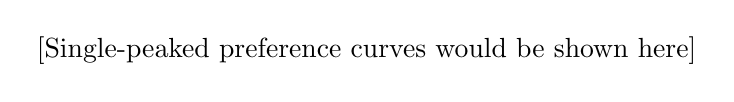
\begin{tikzpicture}[scale=0.8]
  % This is a placeholder for the actual figure
  \node at (0,0) {[Single-peaked preference curves would be shown here]};
\end{tikzpicture}
\end{center}

\subsubsection{Median Voter Theorem}

Under single-peakedness:

\begin{equation}
\boxed{
C^*_{majority} = \text{median voter's ideal point}
}
\label{eq:medianvoter}
\end{equation}

\paragraph{Proof Sketch.}
Median voter's ideal beats any alternative:
\begin{itemize}
    \item Left of median: median + all rightward voters prefer median
    \item Right of median: median + all leftward voters prefer median
\end{itemize}

\subsubsection{Framework Translation}

Single-peakedness is $\Psi$ restriction enabling $C^*$:
\begin{equation}
\Psi_{single-peaked} \Rightarrow \exists C^*_{majority}
\end{equation}

\paragraph{Applications.}
\begin{itemize}
    \item Left-right political spectrum
    \item Tax rate choice
    \item Public good provision level
\end{itemize}

\subsubsection{Moulin: Strategy-Proofness with Single-Peakedness}

Moulin (1980) characterized:

\begin{equation}
\boxed{
\text{Strategy-proof + single-peaked} \Rightarrow \text{Generalized median rules}
}
\label{eq:moulin}
\end{equation}

With single-peaked preferences, strategy-proof mechanisms exist!

%==============================================================================
% PART IV: RIGHTS AND LIBERALISM
%==============================================================================
\subsection{Part IV: Sen's Liberal Paradox – Rights vs. Efficiency}

\subsubsection{The Paradox}

Sen (1970) proved:

\begin{equation}
\boxed{
\text{Pareto Efficiency} + \text{Minimal Liberalism} = \text{Inconsistent}
}
\label{eq:liberal}
\end{equation}

\paragraph{Minimal Liberalism.}
Each person is decisive over at least one pair (their ``private sphere''):
\begin{equation}
\exists (x, y): x \succ_i y \Rightarrow x \succ_{social} y
\end{equation}

\subsubsection{Example}

Two people (Prude, Lewd), one copy of \textit{Lady Chatterley's Lover}:
\begin{itemize}
    \item States: $a$ = Prude reads, $b$ = Lewd reads, $c$ = no one reads
    \item Prude: $c \succ a \succ b$ (prefers no one read, but if someone must, himself)
    \item Lewd: $a \succ b \succ c$ (wants Prude to read to shock him)
\end{itemize}

\paragraph{Liberalism says:}
\begin{itemize}
    \item Prude decides own reading: $c \succ_{social} a$
    \item Lewd decides own reading: $b \succ_{social} c$
\end{itemize}

\paragraph{Pareto says:}
Both prefer $a$ to $b$: $a \succ_{social} b$

\textbf{Cycle}: $a \succ b \succ c \succ a$!

\subsubsection{Framework Translation}

Rights ($\Psi_{rights}$) can conflict with Pareto efficiency:
\begin{equation}
\Psi_{rights} + \Psi_{Pareto} \Rightarrow \nexists C^*_{consistent}
\end{equation}

\paragraph{Implications.}
\begin{itemize}
    \item Individual rights are not just constraints but may conflict with efficiency
    \item Libertarian and welfarist goals can clash
    \item Need to choose which principle takes priority
\end{itemize}

%==============================================================================
% PART V: CAPABILITIES AND WELFARE
%==============================================================================
\subsection{Part V: Sen's Capability Approach – $Q$ Beyond Utility}

\subsubsection{Critique of Utility}

Sen argues utility is inadequate for welfare:
\begin{itemize}
    \item Adaptation: Oppressed people may have low aspirations
    \item Comparison: Utility not interpersonally comparable
    \item Narrow: Misses freedoms, capabilities, agency
\end{itemize}

\subsubsection{Capability Approach}

\begin{equation}
\boxed{
Q = f(\text{Capabilities}) \quad \text{not just } f(\text{Utility})
}
\label{eq:capability}
\end{equation}

\paragraph{Key Concepts.}
\begin{itemize}
    \item \textbf{Functionings}: What people actually do/are (being nourished, educated, mobile)
    \item \textbf{Capabilities}: Set of feasible functionings (freedom to achieve)
    \item \textbf{Agency}: Ability to pursue one's own goals
\end{itemize}

\subsubsection{Framework Translation}

Capabilities enrich $Q$ in FEPSDE:
\begin{equation}
Q_{capability} = \{\text{Feasible functionings}\} \supset Q_{utility}
\end{equation}

\paragraph{FEPSDE Connection.}
\begin{center}
\renewcommand{\arraystretch}{1.3}
\begin{tabular}{|l|l|}
\hline
\textbf{FEPSDE Dimension} & \textbf{Capability Interpretation} \\
\hline
Financial & Economic capability, resource access \\
Emotional & Psychological functioning, autonomy \\
Physical & Health, bodily integrity, mobility \\
Social & Social participation, affiliation \\
Digital & Information access, connectivity \\
Ecological & Environmental quality, sustainability \\
\hline
\end{tabular}
\end{center}

\subsubsection{Development as Freedom}

Sen (1999) argues:

\begin{equation}
\text{Development} = \text{Expansion of capabilities}
\end{equation}

Not just GDP growth, but:
\begin{itemize}
    \item Political freedoms
    \item Economic facilities
    \item Social opportunities
    \item Transparency guarantees
    \item Protective security
\end{itemize}

%==============================================================================
% PART VI: JUDGMENT AGGREGATION
%==============================================================================
\subsection{Part VI: Judgment Aggregation – Beyond Preferences}

\subsubsection{The Problem}

List \& Pettit (2002) extended social choice to beliefs:

\begin{equation}
\boxed{
\text{Aggregate judgments (Yes/No on propositions), not just preferences}
}
\label{eq:judgment}
\end{equation}

\subsubsection{Discursive Dilemma}

Three judges, three propositions:
\begin{itemize}
    \item $p$: Defendant did action
    \item $q$: Action was illegal  
    \item $r$: Defendant is liable (where $r \Leftrightarrow p \land q$)
\end{itemize}

\begin{center}
\begin{tabular}{|c|c|c|c|}
\hline
& $p$ & $q$ & $r$ \\
\hline
Judge 1 & Yes & Yes & Yes \\
Judge 2 & Yes & No & No \\
Judge 3 & No & Yes & No \\
\hline
Majority & Yes & Yes & No \\
\hline
\end{tabular}
\end{center}

Majority says $p$ and $q$, but not $r$---inconsistent with $r \Leftrightarrow p \land q$!

\subsubsection{Framework Translation}

Aggregating $\Psi_K$ (beliefs) faces similar impossibilities:
\begin{equation}
\nexists F: \Psi_K^{collective} = F(\Psi_K^1, \ldots, \Psi_K^n) \text{ preserving consistency}
\end{equation}

\paragraph{Implications.}
\begin{itemize}
    \item Collective rationality is not guaranteed
    \item Organizations may hold inconsistent beliefs
    \item Procedure matters (premise-based vs. conclusion-based)
\end{itemize}

%==============================================================================
% PART VII: STRATEGIC VOTING
%==============================================================================
\subsection{Part VII: Strategic Voting – Sincere vs. Strategic}

\subsubsection{Gibbard-Satterthwaite Revisited}

As in mechanism design (Appendix AE):

\begin{equation}
\boxed{
\text{No strategy-proof, non-dictatorial voting rule with } \geq 3 \text{ alternatives}
}
\label{eq:gs-voting}
\end{equation}

\paragraph{Implication.}
In any reasonable voting system, some voters sometimes benefit from misrepresenting preferences.

\subsubsection{Strategic vs. Sincere Voting}

\begin{equation}
C^*_{strategic} \neq C^*_{sincere} \quad \text{(in general)}
\end{equation}

\paragraph{Examples.}
\begin{itemize}
    \item Plurality: Vote for second choice if first has no chance
    \item Borda: Rank main competitor last
    \item Approval: Strategic threshold choice
\end{itemize}

\subsubsection{Framework Translation}

Voting equilibrium depends on strategic behavior:
\begin{equation}
C^*_{voting} = C^*(\Psi_{voting rule}, \Psi_C^{strategic})
\end{equation}

Sophisticated voters ($\Psi_C$ high) vote strategically.

\subsubsection{Escape Routes}

Barberà (2001) surveys when strategy-proofness is possible:
\begin{itemize}
    \item Single-peaked domains (Moulin 1980)
    \item Randomized mechanisms
    \item Restricted ranges
\end{itemize}

%==============================================================================
% PART VIII: SYNTHESIS
%==============================================================================
\subsection{Part VIII: Synthesis – Social Choice Equations}

\subsubsection{Complete Framework Translation}

\begin{center}
\renewcommand{\arraystretch}{1.5}
\begin{tabular}{|l|c|l|}
\hline
\textbf{Result} & \textbf{Statement} & \textbf{Framework Element} \\
\hline
Arrow & $\nexists F$ with U, P, IIA, ND & Limits on $C^*_{social}$ \\
\hline
Condorcet & Majority cycles possible & $\nexists C^*_{majority}$ sometimes \\
\hline
Median Voter & Single-peaked $\Rightarrow$ median wins & $\Psi_{domain} \to C^*$ exists \\
\hline
Liberal Paradox & Pareto + Rights inconsistent & $\Psi_{rights}$ vs. efficiency \\
\hline
Capabilities & $Q = f(\text{freedoms})$ & $Q$ beyond utility \\
\hline
Judgment Aggregation & Belief aggregation impossible & $\Psi_K^{collective}$ limits \\
\hline
Gibbard-Satterthwaite & No strategy-proof voting & $C^*_{strategic}$ inevitable \\
\hline
\end{tabular}
\end{center}

\subsubsection{The Unified Picture}

Social choice shows:
\begin{equation}
\boxed{
C^*_{social} = f(\Psi_{aggregation}, \text{domain}, \text{constraints})
}
\end{equation}

Key insights:
\begin{enumerate}
    \item \textbf{Aggregation is hard}: Arrow's theorem shows no perfect rule
    \item \textbf{Domain matters}: Single-peakedness enables majority rule
    \item \textbf{Rights conflict}: Liberalism vs. Pareto
    \item \textbf{Welfare is rich}: Capabilities beyond utility
    \item \textbf{Strategy matters}: Voting invites manipulation
\end{enumerate}

\subsubsection{Social Choice's Contribution to Framework}

\textbf{Without Social Choice:}
\begin{itemize}
    \item Assume ``social welfare'' is well-defined
    \item Ignore aggregation problems
    \item Miss rights-efficiency trade-offs
    \item $Q$ limited to utility
\end{itemize}

\textbf{With Social Choice:}
\begin{itemize}
    \item Understand limits of collective $C^*$
    \item Know when voting works (domain restrictions)
    \item Recognize rights as distinct from efficiency
    \item Richer $Q$ via capabilities
    \item Account for strategic behavior
\end{itemize}

%==============================================================================
% PART IX: COMPLETE PAPER DOCUMENTATION
%==============================================================================
\subsection{Part IX: Complete Paper Documentation}

%--- ARROW ---
\subsubsection{Arrow's Theorem}

\paragraph{Paper 1: Arrow (1951/1963)}

\textit{Social Choice and Individual Values.}
Yale University Press. (2nd ed. 1963)

\textbf{Summary.}
Proves impossibility theorem: no social welfare function satisfies unrestricted 
domain, Pareto, IIA, and non-dictatorship with $\geq 3$ alternatives.

\textbf{Framework Translation.}
\begin{equation}
\nexists \Psi_{aggregation} \text{ satisfying all desiderata}
\end{equation}

\textbf{Key Finding.}
Nobel Prize (1972). One of most important results in economics. 15,000+ citations.

\paragraph{Paper 2: Maskin \& Sen (2014)}

\textit{The Arrow Impossibility Theorem.}
Columbia University Press.

\textbf{Summary.}
Modern exposition of Arrow's theorem with new proofs and interpretations.
Accessible introduction with historical context.

\textbf{Framework Translation.}
Contemporary understanding of Arrow's limits.

%--- VOTING THEORY ---
\subsubsection{Voting Theory}

\paragraph{Paper 3: Condorcet (1785)}

\textit{Essai sur l'Application de l'Analyse à la Probabilité des Décisions 
Rendues à la Pluralité des Voix.}

\textbf{Summary.}
Discovers Condorcet paradox (majority cycles) and Condorcet jury theorem 
(majority more likely correct than individuals).

\textbf{Framework Translation.}
\begin{equation}
\text{Majority rule can cycle: } A \succ B \succ C \succ A
\end{equation}

\textbf{Key Finding.}
Foundation of voting theory. 250+ years old.

\paragraph{Paper 4: Black (1948)}

``On the Rationale of Group Decision-Making.''
\textit{Journal of Political Economy}, 56(1), 23--34.

\textbf{Summary.}
Introduces single-peakedness. Shows Condorcet winner exists under 
single-peaked preferences.

\textbf{Framework Translation.}
\begin{equation}
\Psi_{single-peaked} \Rightarrow C^*_{majority} \text{ exists}
\end{equation}

\paragraph{Paper 5: Black (1958)}

\textit{The Theory of Committees and Elections.}
Cambridge University Press.

\textbf{Summary.}
Comprehensive treatment of voting theory. Median voter theorem, 
single-peakedness, history of voting theory.

\textbf{Framework Translation.}
Complete theory of committee voting.

\paragraph{Paper 6: Plott (1967)}

``A Notion of Equilibrium and Its Possibility Under Majority Rule.''
\textit{American Economic Review}, 57(4), 787--806.

\textbf{Summary.}
Shows multidimensional majority rule equilibrium requires extreme symmetry.
Generically, no equilibrium exists.

\textbf{Framework Translation.}
$C^*_{majority}$ rarely exists in multiple dimensions.

\paragraph{Paper 7: McKelvey (1976)}

``Intransitivities in Multidimensional Voting Models and Some Implications 
for Agenda Control.''
\textit{Journal of Economic Theory}, 12(3), 472--482.

\textbf{Summary.}
Proves chaos theorem: in multidimensional voting, majority path connects 
any two points. Agenda setter can reach any outcome.

\textbf{Framework Translation.}
\begin{equation}
\Psi_{agenda} \to C^*_{voting} \quad \text{(agenda determines outcome)}
\end{equation}

\textbf{Key Finding.}
Shows radical instability of majority rule.

%--- SEN ---
\subsubsection{Sen's Contributions}

\paragraph{Paper 8: Sen (1970a)}

\textit{Collective Choice and Social Welfare.}
Holden-Day. (Expanded edition 2017)

\textbf{Summary.}
Comprehensive treatment of social choice. Covers Arrow, voting, 
rights, welfare, capabilities.

\textbf{Framework Translation.}
Foundation for normative framework analysis.

\textbf{Key Finding.}
Nobel Prize (1998). Definitive social choice treatise.

\paragraph{Paper 9: Sen (1970b)}

``The Impossibility of a Paretian Liberal.''
\textit{Journal of Political Economy}, 78(1), 152--157.

\textbf{Summary.}
Proves liberal paradox: minimal liberalism (individual decisive over 
private sphere) conflicts with Pareto efficiency.

\textbf{Framework Translation.}
\begin{equation}
\Psi_{rights} + \Psi_{Pareto} = \text{Inconsistent}
\end{equation}

\textbf{Key Finding.}
5,000+ citations. Shows rights ≠ efficiency.

\paragraph{Paper 10: Sen (1977)}

``Rational Fools: A Critique of the Behavioral Foundations of Economic Theory.''
\textit{Philosophy \& Public Affairs}, 6(4), 317--344.

\textbf{Summary.}
Critiques narrow self-interest assumption. Distinguishes sympathy from 
commitment. People act on values, not just preferences.

\textbf{Framework Translation.}
$\Psi_C$ includes commitments beyond self-interest.

\paragraph{Paper 11: Sen (1999)}

\textit{Development as Freedom.}
Oxford University Press.

\textbf{Summary.}
Argues development is expansion of capabilities, not just GDP growth.
Five instrumental freedoms for development.

\textbf{Framework Translation.}
\begin{equation}
Q_{development} = \text{Capability expansion}
\end{equation}

\textbf{Key Finding.}
Nobel Prize (1998). Influenced UN Human Development Index.

%--- WELFARE ---
\subsubsection{Welfare Theory}

\paragraph{Paper 12: Harsanyi (1955)}

``Cardinal Welfare, Individualistic Ethics, and Interpersonal Comparisons 
of Utility.''
\textit{Journal of Political Economy}, 63(4), 309--321.

\textbf{Summary.}
Derives utilitarian social welfare from impartiality axiom (veil of ignorance).
If equal probability of being anyone, maximize expected utility = sum.

\textbf{Framework Translation.}
\begin{equation}
W = \sum_i U_i \quad \text{(from impartiality)}
\end{equation}

\textbf{Key Finding.}
Nobel Prize (1994). Foundation of modern utilitarianism.

\paragraph{Paper 13: Harsanyi (1977)}

\textit{Rational Behavior and Bargaining Equilibrium in Games and Social Situations.}
Cambridge University Press.

\textbf{Summary.}
Unified treatment of rationality, games, and social welfare. 
Connects individual and collective rationality.

\textbf{Framework Translation.}
Bargaining as social choice mechanism.

\paragraph{Paper 14: Rawls (1971)}

\textit{A Theory of Justice.}
Harvard University Press.

\textbf{Summary.}
Justice as fairness. Original position, veil of ignorance, difference 
principle (maximize welfare of worst-off).

\textbf{Framework Translation.}
\begin{equation}
W = \min_i U_i \quad \text{(maximin from Rawls)}
\end{equation}

\textbf{Key Finding.}
Most influential political philosophy book of 20th century.

%--- STRATEGY-PROOFNESS ---
\subsubsection{Strategy-Proofness}

\paragraph{Paper 15: Gibbard (1973)}

``Manipulation of Voting Schemes: A General Result.''
\textit{Econometrica}, 41(4), 587--601.

\textbf{Summary.}
Proves no non-dictatorial, strategy-proof voting scheme exists with 
$\geq 3$ alternatives.

\textbf{Framework Translation.}
Strategic voting is unavoidable in any reasonable system.

\textbf{Key Finding.}
Foundation of strategic voting theory. [Also in Appendix AE]

\paragraph{Paper 16: Moulin (1980)}

``On Strategy-Proofness and Single Peakedness.''
\textit{Public Choice}, 35(4), 437--455.

\textbf{Summary.}
Characterizes strategy-proof rules under single-peaked preferences.
Generalized median schemes are exactly the strategy-proof rules.

\textbf{Framework Translation.}
\begin{equation}
\Psi_{single-peaked} \Rightarrow \exists \Psi_{strategy-proof}
\end{equation}

\paragraph{Paper 17: Barberà (2001)}

``An Introduction to Strategy-Proof Social Choice Functions.''
\textit{Social Choice and Welfare}, 18(4), 619--653.

\textbf{Summary.}
Survey of strategy-proofness results. When is it achievable? 
Domain restrictions, randomization, range restrictions.

\textbf{Framework Translation.}
Conditions for $C^*_{truthful}$ in voting.

%--- JUDGMENT AGGREGATION ---
\subsubsection{Judgment Aggregation}

\paragraph{Paper 18: List \& Pettit (2002)}

``Aggregating Sets of Judgments: An Impossibility Result.''
\textit{Economics and Philosophy}, 18(1), 89--110.

\textbf{Summary.}
Extends Arrow to judgment aggregation. Shows majority judgment 
on connected propositions can be inconsistent.

\textbf{Framework Translation.}
\begin{equation}
\nexists F: \Psi_K^{collective} = F(\Psi_K^1, \ldots, \Psi_K^n) \text{ consistent}
\end{equation}

\textbf{Key Finding.}
Founded judgment aggregation literature.

\paragraph{Paper 19: List (2012)}

``The Theory of Judgment Aggregation: An Introductory Review.''
\textit{Synthese}, 187(1), 179--207.

\textbf{Summary.}
Survey of judgment aggregation theory. Impossibility theorems, 
escape routes, applications to collective rationality.

\textbf{Framework Translation.}
Complete theory of belief aggregation limits.

%--- TEXTBOOK ---
\subsubsection{Textbook}

\paragraph{Paper 20: Gaertner (2009)}

\textit{A Primer in Social Choice Theory.}
Oxford University Press.

\textbf{Summary.}
Accessible introduction to social choice. Covers Arrow, Sen, voting, 
strategy-proofness, and applications.

\textbf{Framework Translation.}
Modern synthesis of social choice theory.

%%%%%%%%%%%%%%%%%%%%%%%%%%%%%%%%%%%%%%%%%%%%%%%%%%%%%%%%%%%%%%%%%%%%%%%%%%%%%%%
\subsection{Citation and Verification Note}

\textbf{Nobel Prizes represented:}
\begin{itemize}
    \item Arrow (1972) ``for pioneering contributions to general equilibrium theory and welfare theory''
    \item Harsanyi (1994) ``for pioneering analysis of equilibria in non-cooperative games''
    \item Sen (1998) ``for contributions to welfare economics''
\end{itemize}

Combined Google Scholar citations for the 20 papers: $>$100,000.

This appendix provides foundations for understanding collective decision-making 
within the $(C, \Psi, C^*, K, Q)$ framework, including fundamental limits on 
aggregation and richer conceptions of welfare.

%%%%%%%%%%%%%%%%%%%%%%%%%%%%%%%%%%%%%%%%%%%%%%%%%%%%%%%%%%%%%%%%%%%%%%%%%%%%%%%
